
\section{Graph Labeling}
\label{sec:GraphLabeling}

\subsection{Hoshen Kopelman}
\label{subsec:HoshenKopelman}

% TODO: Maybe if I never do XY, change this to the clusters of spins in Ising model
To find the clusters a modified version of the Hoshen Kopelman algorithm was used. A raster scan is used to label disjoint sets into groups with some canonical label\cite{Hoshen:HKAlgo}. It is a variant on the union-find algorithm and is most easily described through the associated functions. Intuitively, applying the find function on a site $i$ returns the canonical, often implemented as the smallest, label in the cluster that $i$ belongs to. Union uses find to ensure that two sites $i$ and $j$ are connected by setting the canonical label of $i$ to that of $j$ (or vice versa). 

An example implementation would be to have a 2D graph without periodic boundary conditions of zeros and ones, where a site is occupied if it has a one associated with it, and unoccupied otherwise. A disjoint set here is a number of occupied sites neighbouring each other with unoccupied sites surrounding them. For simplicity the scan can start in the lower left corner, moving right and up, while search for neighbours left and down, ensuring that if a neighbouring site is occupied, it has been labeled before. 

Start by setting each site to a unique label, putting all sites in individual clusters. Go through the lattice until an occupied site $i$ is found. Search the neighbours below and to the left. If none of these neighbours are occupied, label $i$ have a unique label and move to the next site. If $i$ has one occupied neighbour it must have been labeled before, so $i$ inherits the neighbours label. Finally if both neighbours are occupied, site $i$ must be connecting a cluster and a union is performed on the neighbours to join their labels. A final pass through the lattice using the find function ensures that all sites have their canonical label.

In this paper an occupied site corresponds to a site with connections to the neighbouring sites (in the 2D example above, each site could have four such connections). In the original paper by Hoshen and Kopelman the labels for the sites who did not originally carry the canonical label, were set to a negative integer, symbolizing that they were aliases. A positive value was used at the canonical label, showing the number of sites in that cluster. This was not used in this project since the number of links in a cluster is not necessarily equal to the number of sites.

\section{Fractals}
\label{sec:fractals}

Everyone agrees that the dimension of a point is zero, and that of a smooth line is one, but what about a set of points? A definition could be to say that the dimension is the minimum number of coordinates needed to describe every point in the set. Effectively, a point would describe itself, and a curve could be parametrized to the distance of some point on the same curve.
% TODO: Add this reference to Nonlinear dynamics and chaos with applications to physics, biology, chemistry, and engineering by Steven H. Strogatz
% TODO: Add a plot of the Koch curve.

The situation is more complex when examining fractals. Take for example the Koch curve, it starts out as a line segment of length $L_0$, and successively adds a `bump', making the total length $L_1 = 4/3 \cdot L_0$. Iterating $n$ times gives a line length of $L_n = {(4 / 3)}^n \cdot L_0$, and so the final fractal length is infinite.

Any two point on the final curve has a distance of infinity between them, so parametrization is impossible. But the area is still finite, so the dimension should intuitively be somewhere between one and two.

A useful concept here is the similarity dimension, defined by the scaling of each iteration. If $m$ is the number of similar elements after an iteration and $r$ is the scaling factor, the dimension is defined by $m = r^d$, or equivalently

\begin{equation}
	d = \frac{\ln m}{\ln r}
\end{equation}

So for the Koch curve, each segment is divided into fourths with each having one third the length from the previous iteration, giving it a dimension of $\ln 4 / \ln 3 \approx 1.26$.


\section{Box dimension}
\label{sec:boxdimension}

\section{Graph Dividing Algorithm}
\label{sec:GraphDivisonAlgorithm}

\begin{figure}[h!]
    \centering
        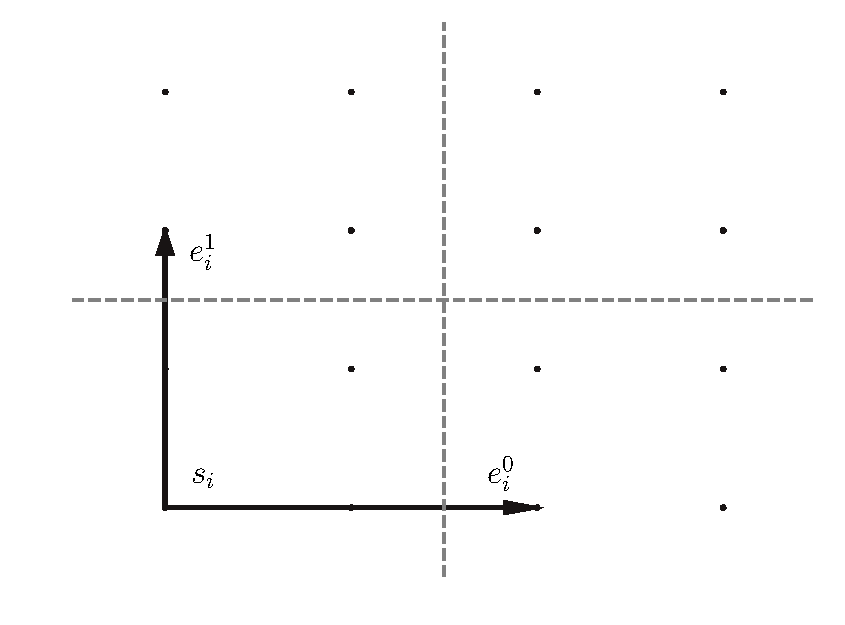
\includegraphics[width=0.6\textwidth]{figures/graphDividing.pdf}
    \caption{One step in the graph dividing algorithm where $l_i = 4$. $e^0_i$ and $e^1_i$ are drawn from site $s_i$. Summed permutations of $\{e^0_i, e^1_i\}$ give the starts for the next boxes. The next iteration of boxes are shown via the dividing dotted lines.}
    \label{fig:graphdividingalgo}
\end{figure}

In order to calculate the box dimension the lattice need to be divided into boxes of decreasing size. A step by step instruction of a graph dividing algorithm is provided below, and an implementation in pseudocode is available in the Appendix at Section \ref{sec:pseudocodeboxdivisionalgo}.

For brevity some abbreviations are introduced.

\begin{equation*}
    \begin{aligned}
        d =& \ \text{dimension} &\quad l_i =& \ \text{side length of the current box}\\
%
        l_0 =& \ \text{side length of the} &\quad e_i^j =& \ \text{vector of length } l_i / 2 \\
%
             & \ \text{smallest box allowed} & & \text{ in the }j\text{'th direction} \\
%
        \text{perm}(v) =& \ \text{All permutations of } v &\quad s_i =& \ \text{starting site of the current box}
    \end{aligned}
\end{equation*}

\begin{enumerate}
    \item If $l_i \geq l_0$, go to 2, else stop.
%
    \item Save all sites in the current box, starting for $s_i$ going $l_i$ in $d$ directions.
%
    \item Find all starting points for new boxes.
%
    \begin{enumerate}[label=(\roman*)]
%
        \item Form the matrix $E = (e_i^0, e_i^1, \  \ldots, e_i^d)^T$
%
        \item For all vectors $v_k$ in perm$(0, 0, \ \ldots , 0)$, perm$(1, 0, \ \ldots , 0)$, \\ \ldots, perm$(1, 1, \ \ldots , 1)$, create the new start $s_k$ as $$s_k = v_k E$$
%
    \end{enumerate}
%
    \item For each start $s_k$:
    \begin{enumerate}[label=(\roman*)]
        \item $s_i = s_k$, $l_i = l_i / 2$
        \item Go to 1.
    \end{enumerate}
%
\end{enumerate}
